%\documentclass[overheadsbeamer.tex]{subfiles}
\documentclass[handoutsbeamer.tex]{subfiles}

\begin{document}

\thispagestyle{empty}

\ona{ \setcounter{chapter}{5} } % ONE LESS
\lecture{The Quantum Approximate Optimization Algorithm}{Lect06}
\chapter{The Quantum Approximate Optimization Algorithm}\label{C.QAOA}

\ona{This \chap{} defines QAOA \cite{farhi2014quantum}, the variational algorithm for combinatorial optimization that the rest of the course studies, establishes that training it is \textbf{NP}-hard \cite{bittel2021training}, and then proves that it nevertheless converges as the depth grows, following the elementary proof of \citet{binkowski2023elementary}, which also covers the constrained \emph{quantum alternating operator ansatz} \cite{hadfield2019quantum}. The first part is adapted from our course on quantum computing \cite{aspman2024quantum}.}

\section{Quantum Approximate Optimization Algorithm}\label{sec:ch06:qaoa}

\begin{frame}\ft{Quantum Approximate Optimization Algorithm}
Variational quantum algorithms can be thought of as quantum randomized algorithms as well, and find many interesting applications. One of the very first applications that sparked the interest of the community is in the context of the Max-Cut problem. Farhi \emph{et al.} introduced the quantum approximate optimization algorithm (QAOA) \cite{farhi2014quantum} as a candidate algorithm to improve upon Max-Cut best bounds, although it is well understood that unless $\textbf{P}=\textbf{NP}$, this is $\textbf{NP}$-hard to achieve. Nevertheless, there is nothing that forbids VQAs to achieve exponential speedups in theory, thus a lot of hope is placed upon them.
\end{frame}

\begin{frame}\ft{MAXCUT}
\ona{\textbf{Max-Cut}} Given a graph $G=(V, E)$ as the input, the Max-Cut problem amounts to finding a partition of the vertex set $V$ into two subsets, $S$ and its complement $V \backslash S$, such that the number of edges going between $S$ and $V \backslash S$ is maximized. That is, we define a cut in the graph $G$ as a pair $(S, V \backslash S)$, where $S \subseteq V$. The edge set of the cut $(S, V \backslash S)$ is
\begin{align*}
    E(S, V \backslash S)=\{e \in E:|e \cap S|=|e \cap(V \backslash S)|=1\}
\end{align*}
\ona{(see Fig. \ref{fig:ch06:maxcut})}, and the size of this cut is $|E(S, V \backslash S)|$, i.e., the number of edges.
\ona{\begin{figure}[htb]
    \centering
    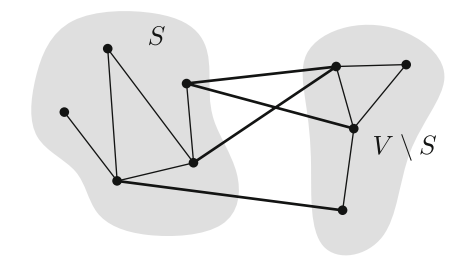
\includegraphics[scale=0.25]{figures/vqa/maxcut.png}
    \caption{An example of a maximum cut (in bold).}
    \label{fig:ch06:maxcut}
\end{figure}}
\onp{\begin{center}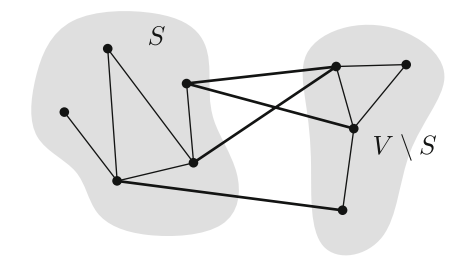
\includegraphics[height=0.3\textheight]{figures/vqa/maxcut.png}\end{center}}
\end{frame}

\begin{frame}\ft{MAXCUT}
\onp{\footnotesize}
\begin{probl}[Max-Cut]\label{p:ch06:maxcut}\hfill
\begin{description}[noitemsep,leftmargin=0.5cm,font=\normalfont]
\item[Instance] An unweighted undirected graph $ G=(V,E) $ represented by an adjacency matrix $ A \in \{0,1\}^{d \times d} $ with the vertex set $ V $ of cardinality $ |V|=d $.
\item[Task] Determine a subset $ S \subseteq V $ that maximizes the size of the cut $ |E(S, V \backslash S)| $, which corresponds to maximizing $ \sum_{i \in S, j \in V \backslash S} A_{i j} $.
\end{description}
\end{probl}
    The decision version of the MaxCut problem is \textbf{NP}-complete\ona{ \cite{Garey1976}}.
The optimization version is \textbf{APX}-hard \ona{\cite{lee2021classifying}} with the optimal (classical) ratio $\alpha_{\rm{max}}=\alpha_{\rm{GW}} \approx 0.878$ of the Goemans--Williamson algorithm \ona{\cite{Goemans1995}} under the assumption that the \emph{Unique Games Conjecture} (UGC) is true. Thus, under UGC, finding a polynomial time algorithm that improves upon the Goemans--Williamson bound is itself a \textbf{NP}-hard problem. However, if the UGC is false, it has been proven that $\alpha_{\max } \leq \frac{16}{17} \approx 0.941$\ona{ \cite{Hstad2001}}.
\end{frame}

\begin{frame}\ft{MAXCUT as an Ising Hamiltonian}
\ona{To run QAOA, we encode a cut by $z \in \{-1,1\}^d$ with $z_i = 1$ iff $i \in S$; then edge $(i,j)$ is cut iff $z_i z_j = -1$, and the cut size is $\frac12\sum_{(i,j)\in E}(1 - z_i z_j)$. Replacing $z_i$ by the Pauli matrix $Z_i$ yields the cost Hamiltonian}
\begin{equation}\label{eq:ch06:HC}
    H_C = -\frac{1}{2}\sum_{(i,j) \in E} w_{ij}\,(\one - Z_i Z_j),
\end{equation}
\ona{which is diagonal in the computational basis with $\braket{x|H_C|x} = -\text{cut}(x)$, so that its ground states are the maximum cuts. QAOA then prepares}
\begin{equation}\label{eq:ch06:qaoa}
    \ket{\psi(\boldsymbol\beta,\boldsymbol\gamma)} = \prod_{k=1}^{p} e^{-i\beta_k H_M}\, e^{-i\gamma_k H_C}\ket{+}^{\otimes n}, \quad H_M = \sum_{j} X_j,
\end{equation}
\ona{and minimises $F_p(\boldsymbol\beta,\boldsymbol\gamma) = \braket{\psi|H_C|\psi}$ over the $2p$ angles. The cost unitary $e^{-i\gamma H_C}$ is a product of two-qubit $ZZ$ rotations, one per edge, and the mixer $e^{-i\beta H_M}$ is a product of single-qubit $X$ rotations.}
\onp{Ground states of $H_C$ are maximum cuts; $e^{-i\gamma H_C}$ is one $ZZ$ rotation per edge; $e^{-i\beta H_M}$ is one $X$ rotation per qubit.}
\end{frame}

\begin{frame}\ft{Depth one is classically easy}
\ona{At $p=1$, the expectation of each edge term $\braket{Z_iZ_j}$ depends only on the neighbourhoods of $i$ and $j$, and has a closed form \cite{farhi2014quantum,Wang2018}. For a $D$-regular triangle-free graph,}
\begin{equation}
    \frac{F_1(\beta,\gamma)}{|E|} = -\frac{1}{2} - \frac{1}{4}\sin(4\beta)\sin(\gamma)\cos^{D-1}(\gamma),
\end{equation}
\ona{which for $D=3$ is optimised at $\beta = \pi/8$, $\gamma = \arctan(1/\sqrt2)$ and gives the ratio $0.6924$ of \citet{farhi2014quantum}. Two consequences: (i) depth-one landscapes can be scanned exactly on a classical computer, which is how iterative angle-setting methods of \Chap~\chref{C.PerIteration} are initialised; (ii) depth one alone is far from GW's $0.878$.}
\onp{\begin{itemize}\item closed form per edge; for 3-regular triangle-free graphs the optimum ratio is $0.6924$ \cite{farhi2014quantum}; \item depth-one landscapes are exactly computable classically \cite{Wang2018}, and far from GW.\end{itemize}}
\end{frame}

\section{VQAs are NP-hard to train}

\begin{frame}\ft{VQAs are \textbf{NP}-hard to train}
An interesting result was given by Bittel and Kliesch \cite{bittel2021training}. To describe this seminal work we can outsource the quantum computation to an oracle $\mathcal{O}$ to avoid potential computational complications associated with the quantum circuit.
\begin{probl}[VQA minimization, oracular formulation]\label{p:ch06:VQAoracle}\hfill
\begin{description}[noitemsep,leftmargin=0.5cm,font=\normalfont]
\item[Instance] A set of Hermitian generators $\{ H_i \}_{i=1,\ldots, L}$ and an observable $O$, given in terms of the Pauli basis representation, acting on $\mathcal{H}$.
\item[Oracle Access] The oracle $\mathcal{O}$ returns the expectation value $\braket{O} \equiv \braket{O(\vartheta)}$ for a given $\vartheta \in \mathbb{R}^L$ up to any desired polynomial additive error $\epsilon$.
\item[Task] Find $\vartheta \in \mathbb{R}^L$ that minimises $\braket{O}$, provided access to the oracle $\mathcal{O}$.
\end{description}
\end{probl}
\ona{The crucial feature of Problem \ref{p:ch06:VQAoracle} is that it captures the complexity of only the classical optimization part of VQAs since the oracle makes the return of the quantum part deterministic.}
\end{frame}

\begin{frame}\ft{VQAs are \textbf{NP}-hard to train}
\begin{thm}[Hardness of VQA optimization, oracular formulation]\label{thm:ch06:NPhard1}
    Assuming \textbf{P}$\neq$\textbf{NP}, there is no deterministic classical algorithm that solves \ona{Prob. \ref{p:ch06:VQAoracle}}\onp{VQA minimization} in polynomial time.
\end{thm}
The proof \ona{of Theorem \ref{thm:ch06:NPhard1}} amounts to reducing the continuous, trigonometric version of MaxCut to \ona{Prob. \ref{p:ch06:VQAoracle}}\onp{VQA minimization}:
\begin{probl}[continuous, trigonometric Max-Cut]\label{p:ch06:triMaxCut}\hfill
\begin{description}[noitemsep,leftmargin=0.5cm,font=\normalfont]
\item[Instance] The adjacency matrix $A \in\{0,1\}^{d \times d}$ of an unweighted undirected graph $G=(V,E)$ with $|V|=d$.
\item[Task] Find $\phi \in[0,2 \pi)^d$ that minimizes
$
\mu(\phi)\coloneqq\frac{1}{4} \sum_{i=1}^d \sum_{j=1}^d A_{i, j}\left(\cos \left(\phi_i\right) \cos \left(\phi_j\right)-1\right).
$
\end{description}
\end{probl}
\ona{One checks that $\mu$ is minimised at $\phi \in \{0,\pi\}^d$, where it equals minus the cut size, and that $\mu(\phi)$ is the energy $\braket{O(\phi)}$ of a product of single-qubit $Y$ rotations applied to $\ket 0^{\otimes d}$ with $O = \frac14\sum_{ij}A_{ij}(Z_iZ_j - \one)$. Hence a single layer of single-qubit gates already suffices for hardness.}
\end{frame}

\begin{frame}\ft{VQAs are \textbf{NP}-hard to train}
\ona{Minima of real valued functions are given by real numbers that may not have an efficient numerical representation. However, it is commonly said that a minimization problem is solved if it is solved to exponential precision, which is the convention we also use. The intuitive notion is that the hardness does not come from the difficulty of representing the minimum.}
The result is robust \cite{bittel2021training}: it persists
\begin{itemize}
    \item when the ansatz uses only logarithmically many qubits,
    \item when it consists of a single layer,
    \item when it is built from free-fermionic gates,
    \item and when time evolution is continuous rather than digitised.
\end{itemize}
Moreover, no polynomial-time algorithm can guarantee an additive optimization error $\Delta < (1-\alpha_{\max})/2$ for QAOA on every instance, where $\alpha_{\max}$ is the best polynomial-time approximation ratio of the underlying problem. \ona{The landscape contains many \emph{persistent} local minima with values bounded away from the optimum \cite{bittel2021training}; see \Chap~\chref{C.PerIteration} for how this is coped with in practice.}
\end{frame}


\ona{\section*{Convergence of QAOA}}
\begin{frame}\ft{Does it converge?}
\ona{We know that training QAOA to optimality is hard. A separate question is whether the ansatz is \emph{expressive} enough: is there, for every instance, a depth $p$ and angles such that $\ket{\vec\beta,\vec\gamma}$ is close to an optimal solution? \citet{farhi2014quantum} sketched an argument via the adiabatic theorem (\Chap~\chref{C.Annealing}); \citet{binkowski2023elementary} make it rigorous and general. The rest of this \chap{} follows their proof. We switch to maximisation, which makes the statements more compact.}
\onp{Expressivity: for every instance, is there a depth and angles reaching the optimum? Yes, via the adiabatic theorem; we prove it, following \citet{binkowski2023elementary}.}
\end{frame}

\section{Setting}

\begin{frame}\ft{Combinatorial optimization problems and their encoding}
\ona{We restrict to maximisation, which makes the proofs read more compactly. A generic combinatorial optimization problem (COP) of size $N$ is}
\begin{equation}\label{eq:ch06c:cop}
    \max_{\boldsymbol z \in S} f(\boldsymbol z), \qquad S \subseteq \{0,1\}^N,
\end{equation}
\ona{with objective $f$ and feasible set $S$; the problem is unconstrained if $S = \{0,1\}^N$; $S_{\max}$ denotes the set of maximisers. Encoding on $N$ qubits, $\mathcal H = \C^{2^N}$:}
\begin{align}
    C &\coloneqq \sum_{\boldsymbol z} f(\boldsymbol z)\,\ket{\boldsymbol z}\!\bra{\boldsymbol z} && \text{(objective Hamiltonian)},\\
    \mathcal S &\coloneqq \spn\{\ket{\boldsymbol z} : \boldsymbol z \in S\}, \quad
    \mathcal S_{\max} \coloneqq \spn\{\ket{\boldsymbol z} : \boldsymbol z \in S_{\max}\} && \text{(solution spaces)}.
\end{align}
\ona{$\mathcal S_{\max}$ is the eigenspace of $C|_{\mathcal S}$ for its largest eigenvalue, and we consider \emph{any} highest-energy state of $C|_{\mathcal S}$ an optimal solution.}
\end{frame}

\begin{frame}\ft{QAA and QAOA}
\ona{The \emph{quantum adiabatic algorithm} (QAA) evolves an initial state $\ket\iota$, a highest-energy state of $H_{\rm init}$, under the linear interpolation}
\begin{equation}\label{eq:ch06c:interp}
    H_{\rm lin(H_{\rm init}, C)}(t) \coloneqq (1-t)\,H_{\rm init} + t\,C, \qquad t \in [0,1],
\end{equation}
\ona{slowed down by a parameter $T$: the actual evolution is under $H(s/T)$ for $s \in [0,T]$. The \emph{quantum approximate optimization algorithm} \cite{farhi2014quantum} fixes $\ket\iota = \ket{+}^{\otimes N}$, the non-degenerate highest-energy state of $B = \sum_n X^{(n)}$, and prepares}
\begin{equation}\label{eq:ch06c:qaoa}
    \ket{\vec\beta,\vec\gamma} \coloneqq \Big(\prod_{q=1}^{p} U_B(\beta_q) U_C(\gamma_q)\Big)\ket{+}^{\otimes N}, \qquad U_B(\beta) = e^{-i\beta B},\ U_C(\gamma) = e^{-i\gamma C},
\end{equation}
\ona{optimising $F_p(\vec\beta,\vec\gamma) = \braket{\vec\beta,\vec\gamma|C|\vec\beta,\vec\gamma}$. The \emph{quantum alternating operator ansatz} \cite{hadfield2019quantum} replaces $U_B$ by a problem-specific mixer $U_M$ that (i) preserves feasibility, $U_M(\beta)\mathcal S \subseteq \mathcal S$, and (ii) mixes fully: for all feasible $\ket{\boldsymbol z},\ket{\boldsymbol z'}$ there are $r, \beta$ with $\braket{\boldsymbol z|U_M^r(\beta)|\boldsymbol z'} \ne 0$.}
\onp{QAA: adiabatic evolution along \eqref{eq:ch06c:interp}. QAOA: discrete alternation \eqref{eq:ch06c:qaoa}. Alternating operator ansatz: any feasibility-preserving, fully mixing $U_M$ instead of $U_B$.}
\end{frame}

\begin{frame}\ft{Phase separators}
\begin{defn}[Phase separator]\label{def:ch06c:phase}
Given a COP with solution space $\mathcal S$ and optimal solution space $\mathcal S_{\max}$, a Hamiltonian $H$ is a \emph{phase separator Hamiltonian} iff (i) $H$ is diagonal in the computational basis, and (ii) the eigenspace of $H|_{\mathcal S}$ for its largest eigenvalue is $\mathcal S_{\max}$. The corresponding parametrised phase separator is $U_P(H,\gamma) \coloneqq e^{-i\gamma H}$.
\end{defn}
\ona{The objective Hamiltonian $C$ is a phase separator, but so is any diagonal Hamiltonian that ranks the feasible solutions in the same way at the top. Diagonality is what makes the convergence proof go through: adding a diagonal matrix does not destroy irreducibility.}
\end{frame}

\section{Convergence of the QAA}

\begin{frame}\ft{Two theorems from the shelf}
\begin{thm}[Adiabatic theorem without gap condition, \citet{Teufel2001}]\label{thm:ch06c:adiabatic}
Let $H(\cdot) \in C^2([0,1], \mathcal L(\mathcal H))$ be self-adjoint, $U_T(t)$ the evolution under $H(s/T)$ rescaled to $t \in [0,1]$, $\lambda(t)$ an eigenvalue of $H(t)$ with spectral projection $\mathbb P(t)$, and $P \in C^2([0,1],\mathcal L(\mathcal H))$ a family of projections with $H(t)P(t) = \lambda(t)P(t)$ and $P(t) = \mathbb P(t)$ for almost all $t$. Then
$\lim_{T\to\infty} (\one - P(t))\,U_T(t)\,P(0) = 0$ uniformly in $t$.
\end{thm}
\ona{In words: starting in the eigenspace of $\lambda(0)$, one stays in the eigenspace of $\lambda(t)$ in the adiabatic limit, provided the projections can be continued $C^2$-smoothly \emph{through} level crossings. \citet{farhi2014quantum} used the classical version that forbids crossings altogether.}
\begin{thm}[Perron--Frobenius]\label{thm:ch06c:pf}
A component-wise non-negative, irreducible matrix $A \in \C^{n\times n}$ has a non-degenerate largest eigenvalue.
\end{thm}
\ona{Recall that $A$ is \emph{irreducible} iff the only coordinate subspaces it leaves invariant are $\{0\}$ and $\C^n$; equivalently, the graph with adjacency pattern of $A$ is strongly connected.}
\end{frame}

\begin{frame}\ft{Mixers}
\begin{defn}[Mixer]\label{def:ch06c:mixer}
A Hamiltonian $B \in \mathcal L(\mathcal H)$ is a \emph{mixer} for a COP with solution space $\mathcal S$ iff $B\mathcal S \subseteq \mathcal S$ and $B|_{\mathcal S}$ is component-wise non-negative and irreducible in the computational basis.
\end{defn}
\begin{itemize}\setlength\itemsep{0.2em}
    \item The transverse field $B = \sum_n X^{(n)}$ is a mixer for unconstrained problems: its matrix is the adjacency matrix of the hypercube, which is connected and non-negative.
    \item The conditions are exactly those of Perron--Frobenius, and they survive adding a diagonal matrix:
\end{itemize}
\begin{cor}\label{cor:ch06c:irred}
If $A$ is diagonal and $B$ is irreducible, then $A + B$ is irreducible.
\end{cor}
\ona{Indeed, a coordinate subspace invariant under $A+B$ is invariant under $B$, since $A$ leaves every coordinate subspace invariant.}
\end{frame}

\begin{frame}\ft{Convergence of the QAA}
\begin{thm}[Convergence of QAA, \citet{binkowski2023elementary}]\label{thm:ch06c:qaa}
Consider a COP with solution space $\mathcal S$, optimal solution space $\mathcal S_{\max}$, and phase separator Hamiltonian $C$. If $B$ is a mixer and $\ket\iota \in \mathcal S$ is a highest-energy state of $B|_{\mathcal S}$, then
\begin{equation}
    \lim_{T\to\infty} U_T(1)\ket\iota \in \mathcal S_{\max},
\end{equation}
where $U_T$ is the quasi-adiabatic evolution along the linear interpolation between $B$ and $C$.
\end{thm}
\ona{Note what is \emph{not} assumed: the optimum need not be unique. \citet{farhi2014quantum} assumed uniqueness to rule out a level crossing at $t = 1$; the gapless adiabatic theorem makes this unnecessary.}
\end{frame}

\begin{frame}\ft{Proof of Theorem~\ref{thm:ch06c:qaa}}
\onp{\scriptsize}
\ona{Work in $\mathcal L(\mathcal S)$ with matrices in the computational basis, and let $\lambda_{\max}(t)$ be the largest eigenvalue of $H(t) \coloneqq (1-t)B|_{\mathcal S} + tC|_{\mathcal S}$.}
\begin{enumerate}\setlength\itemsep{0.2em}
    \item \emph{Non-degeneracy for $t<1$.} For $0 \le t_0 < 1$, $(1-t_0)B|_{\mathcal S}$ is irreducible and non-negative; $C$ is diagonal, and w.l.o.g.\ has non-negative spectrum (shift both $B$ and $C$ by $-\lambda_{\min}\one$, which changes the evolution by a global phase). By Corollary~\ref{cor:ch06c:irred}, $H(t_0)$ is non-negative and irreducible, so by Perron--Frobenius $\lambda_{\max}(t_0)$ is non-degenerate.
    \item \emph{Analytic continuation.} $t \mapsto H(t)$ is analytic and symmetric, so by Kato's perturbation theory \cite{Kato1995} the eigenvalues can be sorted into analytic curves $\lambda_m(t)$ whose spectral projections $\mathbb P_m(t)$ are analytic away from the discrete set $L$ of crossings and have removable singularities there; the continuations $P_m$ are projections of constant rank with $H(t)P_m(t) = \lambda_m(t)P_m(t)$ for all $t$.
    \item \emph{Identify the top curve.} Let $\lambda_1(0) = \lambda_{\max}(0)$. Since $\lambda_{\max}(t_0)$ is non-degenerate on $[0,1)$, $\lambda_1 \equiv \lambda_{\max}$ there, and by continuity also at $t = 1$. Its projection $P_1$ satisfies the hypotheses of Theorem~\ref{thm:ch06c:adiabatic}.
    \item \emph{Conclude.} $P_1(0)\ket\iota = \ket\iota$, so $\lim_T (\one - P_1(1))U_T(1)\ket\iota = 0$, i.e.,
    $\lim_T U_T(1)\ket\iota = P_1(1)\lim_T U_T(1)\ket\iota$, which lies in $\operatorname{im} P_1(1) \subseteq \mathcal S_{\max}$. \qed
\end{enumerate}
\onp{Perron--Frobenius $\Rightarrow$ top eigenvalue simple for $t<1$; Kato $\Rightarrow$ analytic eigen-curves through the crossing at $t=1$; gapless adiabatic theorem $\Rightarrow$ the state follows the top curve.}
\end{frame}

\begin{frame}\ft{Level crossings only at the end}
\ona{The top eigenvalue curve $\lambda_{\max}$ is separated from all others for $0 \le t < 1$. If the COP has a unique optimum the separation extends to $t=1$; with multiple optima, $\lambda_{\max}$ meets at least one other curve exactly at $t = 1$, see Fig.~\ref{fig:ch06c:crossing}. The crossing happens once, at a predictable time, which is why a gapless adiabatic theorem suffices.}
\begin{center}
\begin{tikzpicture}[scale=1.3]
  \draw[->] (0, 0) -- ++(3, 0) node[right] {$t$};
  \draw (0, 0) -- ++(0,-0.05) node[below] {$0$};
  \draw (2.8, 0) -- ++(0,-0.05) node[below] {$1$};
  \draw[->] (0, 0) -- (0, 3) node[above] {$\{\lambda_{i}(t)\}_{i}$};
  \draw[scale=2.8, domain=0:1, smooth, variable=\x, red] plot ({\x}, {0.8-0.2*sin(2.5*\x*\x r)});
  \draw[scale=2.8, domain=0:1, smooth, variable=\y] plot ({\y*\y}, {0.3+0.2*\y*\y*\y});
  \node at (1.5,2.1) {\footnotesize \color{red}$\lambda_{\max}$};
\end{tikzpicture}
\hspace{1cm}
\begin{tikzpicture}[scale=1.3]
  \draw[->] (0, 0) -- ++(3, 0) node[right] {$t$};
  \draw (0, 0) -- ++(0,-0.05) node[below] {$0$};
  \draw (2.8, 0) -- ++(0,-0.05) node[below] {$1$};
  \draw[->] (0, 0) -- ++(0, 3) node[above] {$\{\lambda_{i}(t)\}_{i}$};
  \draw[scale=2.8, domain=0:1, smooth, variable=\x, red] plot ({\x}, {0.8-0.2*sin(2.5*\x*\x r)});
  \draw[scale=2.8, domain=0:1, smooth, variable=\y] plot ({\y}, {0.3+0.38*\y*\y*\y});
  \node at (1.5,2.1) {\footnotesize \color{red}$\lambda_{\max}$};
\end{tikzpicture}
\end{center}
\ona{\begin{figure}[htb]\caption{The eigenvalue curve $\lambda_{\max}$ stays separated from all other curves for $0 \le t < 1$. With a unique optimum the separation extends to $t=1$ (left); with multiple optima $\lambda_{\max}$ intersects another curve at $t=1$ (right). After \citet{binkowski2023elementary}.}\label{fig:ch06c:crossing}\end{figure}}
\end{frame}

\section{Convergence of the QAOA}

\begin{frame}\ft{Mixing families}
\ona{Applications decompose the mixer into local terms, and the alternating operator ansatz exponentiates them separately. The right notion is:}
\begin{defn}[Mixing family]\label{def:ch06c:family}
A family $\{B_i\}_{i\in I} \subset \mathcal L(\mathcal H)$ is a \emph{mixing family} for a COP with solution space $\mathcal S$ iff each $B_i\mathcal S \subseteq \mathcal S$, each $B_i|_{\mathcal S}$ is component-wise non-negative, and any coordinate subspace of $\mathcal S$ invariant under \emph{every} $B_i$ is trivial.
\end{defn}
\begin{propn}\label{prop:ch06c:family}
$\{B_i\}_{i\in I}$ is a mixing family iff $B_I \coloneqq \sum_{i\in I} B_i$ is a mixer.
\end{propn}
\ona{View each $B_i|_{\mathcal S}$ as the adjacency matrix of a graph $G_i$ on the feasible basis states. Non-negativity means no cancellations in the sum, so the graph of $B_I$ is the union of the $G_i$; triviality of common invariant coordinate subspaces means this union is connected, i.e., $B_I$ is irreducible. See Fig.~\ref{fig:ch06c:family}.}
\end{frame}

\begin{frame}\ft{Mixing families: illustration}
\begin{center}
\begin{tikzpicture}[scale=0.75, every node/.style={scale=0.85}]
    \node (z11) at (0,0) {$\ket{\boldsymbol z_{1}}$};
    \node (z21) at (2.5,0) {$\ket{\boldsymbol z_{2}}$};
    \node (z31) at (0,-2.5) {$\ket{\boldsymbol z_{3}}$};
    \node (z41) at (2.5,-2.5) {$\ket{\boldsymbol z_{4}}$};
    \draw (z11.east) -- (z21.west);
    \draw (z31.east) -- (z41.west);
    \node at (1.25,-3.3) {$G_{1}$};
    \node at (4,-1.25) {\Large $\cup$};
    \node (z12) at (5.5,0) {$\ket{\boldsymbol z_{1}}$};
    \node (z22) at (8,0) {$\ket{\boldsymbol z_{2}}$};
    \node (z32) at (5.5,-2.5) {$\ket{\boldsymbol z_{3}}$};
    \node (z42) at (8,-2.5) {$\ket{\boldsymbol z_{4}}$};
    \node at (6.75,-3.3) {$G_{2}$};
    \draw (z12.south) -- (z32.north);
    \draw (z32.east) -- (z42.west);
    \node at (9.5,-1.25) {\Large $=$};
    \node (z13) at (11,0) {$\ket{\boldsymbol z_{1}}$};
    \node (z23) at (13.5,0) {$\ket{\boldsymbol z_{2}}$};
    \node (z33) at (11,-2.5) {$\ket{\boldsymbol z_{3}}$};
    \node (z43) at (13.5,-2.5) {$\ket{\boldsymbol z_{4}}$};
    \draw (z13.east) -- (z23.west);
    \draw (z13.south) -- (z33.north);
    \draw (z33.east) -- (z43.west);
    \node at (12.25,-3.3) {$G_{I}$};
\end{tikzpicture}
\end{center}
\ona{\begin{figure}[htb]\caption{Proof of Proposition~\ref{prop:ch06c:family}. The feasible subspace is spanned by $\ket{\boldsymbol z_1},\dots,\ket{\boldsymbol z_4}$. $B_1$ leaves $\spn\{\ket{\boldsymbol z_1},\ket{\boldsymbol z_2}\}$ and $\spn\{\ket{\boldsymbol z_3},\ket{\boldsymbol z_4}\}$ invariant; $B_2$ leaves $\spn\{\ket{\boldsymbol z_1},\ket{\boldsymbol z_3},\ket{\boldsymbol z_4}\}$ and $\spn\{\ket{\boldsymbol z_2}\}$ invariant; they share no proper invariant coordinate subspace, hence $B_1 + B_2$ is a mixer. After \citet{binkowski2023elementary}.}\label{fig:ch06c:family}\end{figure}}
\onp{No common proper invariant coordinate subspace $\Leftrightarrow$ the union graph is connected $\Leftrightarrow$ $B_1 + B_2$ is a mixer.}
\end{frame}

\begin{frame}\ft{Simultaneous and sequential mixers}
\begin{defn}\label{def:ch06c:mixers}
Let $\mathsf H = \{H_i\}_{i\in I}$ be a mixing family. The \emph{simultaneous mixer} and, for a permutation $\sigma$ of $I$, the \emph{sequential mixer} are
\begin{equation}
    U_M^{\rm sim}(\mathsf H,\beta) \coloneqq e^{-i\beta\sum_{i\in I}H_i}, \qquad
    U_M^{\rm seq}(\mathsf H,\beta) \coloneqq \prod_{i\in I} e^{-i\beta H_{\sigma(i)}}.
\end{equation}
\end{defn}
\ona{Both fulfil the original demands of feasibility preservation and full mixing. The sequential mixer is what one implements: e.g., the $XY$ mixer for Hamming-weight constraints as a product of two-qubit exponentials, or the transverse field as a product of single-qubit $X$ rotations.}
\begin{lem}[Products of nearby unitaries]\label{lem:ch06c:product}
If $\|V_j - W_j\| < \varepsilon$ for unitaries $V_j, W_j$, $j = 1,\dots,m$, then $\big\|\prod_j V_j - \prod_j W_j\big\| < (1+\varepsilon)^m - 1$.
\end{lem}
\ona{Proof by induction: write $V_j = W_j + \varepsilon R_j$ with $\|R_j\| \le 1$; the product with $m+1$ factors differs from the one with $m$ factors by at most $\varepsilon \cdot \|\prod_{j\le m} V_j\| \le \varepsilon(1+\varepsilon)^m$.}
\end{frame}

\begin{frame}\ft{Convergence of the QAOA}
\begin{thm}[Convergence of QAOA, \citet{binkowski2023elementary}]\label{thm:ch06c:qaoa}
Consider a COP with solution space $\mathcal S$, optimal solution space $\mathcal S_{\max}$, phase separator Hamiltonian $C$, and mixing family $\{B_i\}_{i\in I}$; let $U_P$ and $U_M$ be the corresponding phase separator and (simultaneous or sequential) mixer, and $\ket\iota \in \mathcal S$ a highest-energy state of $B_I|_{\mathcal S}$. Then for every $\varepsilon > 0$ there are finitely many parameters $\vec\beta,\vec\gamma$ such that
\begin{equation}
    \dist\big(\ket{\vec\beta,\vec\gamma},\ \mathcal S_{\max}\big) < \varepsilon, \qquad
    \ket{\vec\beta,\vec\gamma} \coloneqq \Big(\prod_q U_M(\beta_q)U_P(\gamma_q)\Big)\ket\iota.
\end{equation}
\end{thm}
\ona{This contains the original QAOA (unconstrained, $B = \sum X^{(n)}$, $\ket\iota = \ket{+}^{\otimes N}$) and the warm-started QAOA of \Chap~\chref{C.WSRounded} whose mixer has the warm initial state as ground state, but \emph{not} the rounded warm start with the modified mixer, where the initial state is not an eigenstate of the mixer.}
\end{frame}

\begin{frame}\ft{Proof of Theorem~\ref{thm:ch06c:qaoa}}
\ona{Three steps: discretise the adiabatic evolution, split each step by a Lie product formula, and invoke Theorem~\ref{thm:ch06c:qaa}.}
\begin{enumerate}\setlength\itemsep{0.2em}
    \item By Proposition~\ref{prop:ch06c:family} $B_I$ is a mixer, so Theorem~\ref{thm:ch06c:qaa} gives $T$ with $\|(\one - P_1(1))U_T(1)\ket\iota\| < \varepsilon/2$. Let $\alpha \coloneqq \|\one - P_1(1)\| > 0$ (assume $\dim\mathcal S > 1$).
    \item \emph{Discretise:} there is $m$ with $\big\|\prod_{j=1}^m W_j - U_T(1)\big\| < \varepsilon/(4\alpha)$, where $W_j \coloneqq \exp\!\big(-i\,H_{\rm lin}(j\tfrac{T}{m})\,j\tfrac{T}{m}\big)$.
    \item \emph{Split:} by the (multivariate) Lie product formula, there is $n$ such that for all $j$,
    \begin{equation*}
        \Big\|\Big(\prod_{i\in I} e^{-i\frac{1-jT/m}{n}\,\frac{jT}{m}B_i}\ e^{-i\frac{(jT/m)^2}{n}C}\Big)^{n} - W_j\Big\| < \sqrt[m]{\tfrac{\varepsilon}{4\alpha}+1} - 1,
    \end{equation*}
    and similarly with $e^{-i(\cdots)B_I}$ for the simultaneous mixer. Each factor is $U_M(\beta)U_P(\gamma)$ for explicit angles $\beta = \frac{(1-jT/m)}{n}\frac{jT}{m}$, $\gamma = \frac{(jT/m)^2}{n}$; there are $q = nm$ layers.
    \item By Lemma~\ref{lem:ch06c:product}, $\|V(\vec\beta,\vec\gamma) - \prod_j W_j\| < \varepsilon/(4\alpha)$, hence $\|V(\vec\beta,\vec\gamma) - U_T(1)\| < \varepsilon/(2\alpha)$, and
    $\|(\one - P_1(1))\ket{\vec\beta,\vec\gamma}\| \le \alpha\cdot\frac{\varepsilon}{2\alpha} + \frac\varepsilon2 = \varepsilon$. Since $\operatorname{im}P_1(1) \subseteq \mathcal S_{\max}$, done. \qed
\end{enumerate}
\end{frame}

\section{Discussion}

\begin{frame}\ft{What the proof gives, and what it does not}
\begin{itemize}\setlength\itemsep{0.3em}
    \item \textbf{Fewer assumptions.} Multiple optima are allowed; non-trivial feasibility structures $\mathcal S \subsetneq \mathcal H$ are covered; sequential mixers are covered.
    \item \textbf{Sharp definitions.} Irreducibility of $B|_{\mathcal S}$ is \emph{necessary} in the sense that with a non-trivial invariant coordinate subspace there is an objective for which neither QAA nor QAOA can approximate an optimum. Component-wise non-negativity is sufficient but not necessary; more general Perron--Frobenius theorems for cone-preserving maps lead essentially back to the same conditions.
    \item \textbf{The same notions recur} when one encodes classical feasibility symmetries into QAOA, which suggests they capture the principle correctly.
    \item \textbf{No rate.} The proof is existential: the angles come from a Trotterised adiabatic schedule with $q = nm$ layers, and nothing is said about how large $q$ must be. Rates would require gap estimates, which vanish at $t\to1$ with multiple optima; results on the rate in gapless adiabatic theorems are a promising avenue.
\end{itemize}
\ona{The existential nature of the guarantee is exactly why the practical questions of \Chaps~\chref{C.IterationComplexity}--\chref{C.WSRounded} matter: at fixed small depth, everything depends on how the angles are chosen and where one starts.}
\end{frame}


\begin{frame}[allowframebreaks]\ft{References}
\biblio
\end{frame}

\end{document}
